\section{Performance test}

A modified version of Fitts' Law will be used to quantify the performance of the trained regressors. Fitts' Law is a predictive model describing the relation that the time it takes to do a rapid movement to reach a target area, is dependent on the distance to the target area, and the size of the target area. The law demonstrates that the information of any human motor tasks, is finite and only limited by the capabilities of the control system. The control exhibit a negative correlation between speed and accuracy. \cite{Kamavuako2014}
Fitts' Law calculates an \textit{Index of Difficulty} (ID) by \eqref{eq:Fitts}

\begin{equation} \label{eq:Fitts}
ID = log_{2} * (\frac{2D}{W})
\end{equation}

Where ID is Index of Difficulty, D is distance to targes and W is width of target area. However, the system in this study does not provide a reasonable scale for distance and target width. Thus, Fitts' Law cannot be used as usual. Instead only the time is takes a subject to reach the targets and the number of targets reached will be noted to calculate a performance score. The score will be calculated as shown in \eqref{eq:ourScore}.

\begin{equation} \label{eq:ourScore}
	Score = \frac{time}{targets\ reached}
\end{equation}

The equation indicates that the lower the score the better the performance.

This modified Fitts' Law test will be implemented in the test GUI compass-plot, as seen in \figref{fig:PlacesToGo}. 

\begin{figure}[H]
	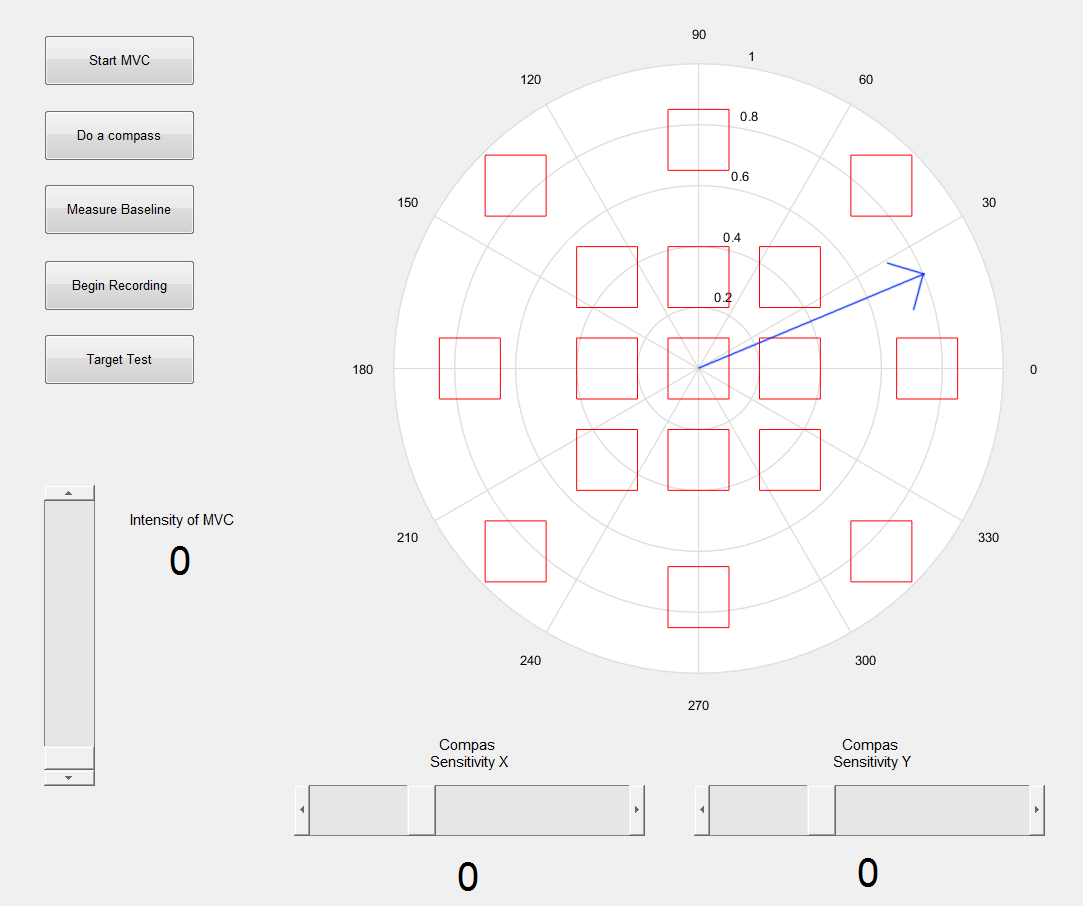
\includegraphics[width=1\textwidth]{figures/Methods/PlacesToGo.png}  %<--but is not needed.
	\caption{The compass plot shows the performed movements and the given intensity of the EMG depicted as an arrow originated in origo. The direction of the arrow decides the movement and the length decides the intensity. The test GUI is implemented in the same GUI as the training GUI, but the plot will change once the "target test" button is pressed. The red squares are targets the subject needs to reach. Only one target will be present at a time, but all the targets are depicted in this illustration to show which targets the subjects will be asked to reach.}
	\label{fig:PlacesToGo}
\end{figure}

The test will consist of reaching 16 targets on time. Each target will be present for 45 seconds. If a target is not reached within that time the test will mark the target as missed and move on to the next target. The targets are oriented around origin in two different radii: eight targets close to origin and eight further away. This is done in order to test the proportional control of the regressors. The targets will be fixed on the axes of the compass-plot and in the diagonals in order to test for simultaneous control. 
During evaluation of the performance score it will be analysed which targets were reached. This can provide knowledge on the regressors if there are specific directions in which they perform worse, due to targets not reached in that quadrant. 


%To calculate the performance of the human interacting with the control system, the \textit{throughput} (TP) was introduced. IP is calculated by \eqref{eq:TP}.
%
%\begin{equation} \label{eq:TP}
%TP = \frac{ID}{MT}
%\end{equation}
%
%where ID is Index of Difficulty, MT is movement time.
%MT is the time it would take a subject to move a pointer from origin to the target area.
%
%Fitts' Law will be implemented into the test GUI described in \secref{sec:testGUI}, where it will test the control systems ability to correctly convey the test subjects task of reaching points in the compass-plot.
